\graphicspath{
%{PHD/analyses_Guillaume/Figures-Resultat/Fluo/}
{PHD/Etudes/GHD/Yang-Yang/Figures/}
}

\section{C'est quoi la temperature des nuage ?}
\begin{frame}[shrink=20]{Methode}
	
	\begin{itemize}
		\item[Contexte :]  Dans les scans du 29 mai 2023 et autres, nous avons produit des gaz quantiques en mesurant les paramètres $\omega_\perp$ et $\omega_\parallel$. Dans tous ces scans, nous avons fait varier les deux paramètres.
		\item[Objectif :] Mesurer la température de ces nuages.
		\item[Théorie :]	Yang-Yang
		\item[Méthod :]	
			\begin{itemize}
				\item[$\rhd$] Ajuster le profil longitudinal avec $ n(z)  = \frac{1}{4 a_{3D}} \left (  \left ( k_B \frac{ \mu_p - \frac{1}{2} m \omega_ \parallel^2 (z-z_0)^2 }{\hbar \omega_\perp} + 1 \right )^2 - 1 \right ) $ pour avoir :  
					\begin{itemize}
						\item[$\circ$] $n_p$ (, $z_0$)
						\item[$\bullet$] $\omega_\perp$ , $\omega_ \parallel$ (première vérification)
					\end{itemize} 
				\item[$\rhd$] Ajuster le profil longitudinal avec la thèorie de Yang-Yang 
					\begin{itemize}
						\item[1] variables : libre T ; fixe : $\omega_\perp$ , $\omega_\parallel$ , $z_0$ , $\mu_p$ (mesurés)
						\item[2] variables : libre $\omega_\parallel$ , T ; fixe : $\omega_\perp$ , $z_0$ , $\mu_p$ ~(vérif $\omega_\parallel$ )
						\item[3] variables : libre $\omega_\parallel$ , T  , $\mu_p$ ; fixe : $\omega_\perp$ ,  $z_0$
						\item[4] variables : libre $\omega_\perp$ , $\omega_\parallel$ , T , $\mu_p$; fixe :  $z_0$ 
						\item[5] variables : libre $\omega_\perp$ , $\omega_\parallel$ ,$z_0$  ,  T , $\mu_p$; fixe :  
					\end{itemize} 
			\end{itemize} 
		\item[ Précaussions ]  :
			\begin{itemize}
				\item[$\bullet$] On selection que le centre du nuage pour faire l'ajustement "Thomas-Fermi". 
				\item[$\bullet$] On ne selection que les bors du nuage pour faur l'ajustement "Yang-Yang" [Max]
			\end{itemize} 
	\end{itemize}  
	


	
\end{frame}


\begin{frame}[shrink=1]{Données du 2023-05-02-Scan-29  fit \only<1-2>{ Thomas-Fermi , }\only<2->{Yang-Yang}}
	
	\only<1-2>{
	{~}\\
	\begin{columns}
	
		\begin{column}{0.3\linewidth}		
			$$ 
			{\tiny 
			\begin{array}{rrl}
				\hline
				\hline
				n_p:  & 127.83  & {\mu m}^{-1}\\
				\omega_\perp :  & 2 \pi  \times 2.589  & kHz	\\
				\omega_\parallel :  & 2 \pi  \times 7.815  & Hz	\\
				z_0 :  &  462.19 & \mu m	\\
				\hline
				\hline
				\mu_p : & 0.1152 & \mu K \\ 
				\hline
				\hline	
				\frac{ k_B \mu_p}{\hbar \omega_\perp } :  &  0.928  & 	\\
				n_p a_{3D} :  & 0.68  &  \\
				\hline
				\hline
			\end{array}
			}
			$$
		
		\end{column}
		
		
		\begin{column}{0.7\linewidth}	
			\centering
			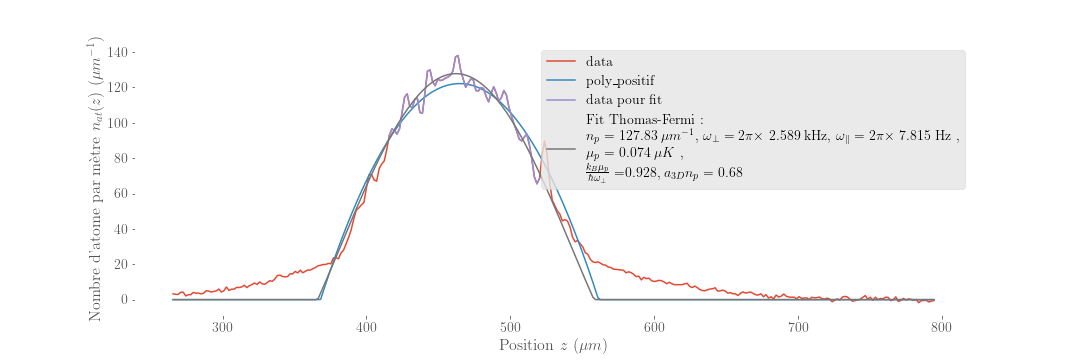
\includegraphics[width=0.99\textwidth]{n_at_2023-05-02-Scan-29_Thomas-Fermi}
		
		\end{column}


		
	\end{columns}
	}
	
	\only<1>{\tiny
			$$  \mu_p = \frac{1}{k_B} \hbar  \omega_\perp  (\sqrt { 1 + 4  n_p  a_{3D} } - 1 )$$ } 
	
	\only<2>{
	{~}\\
	{~}\\
	{$\bullet$ Paramètre libre {\color{red}$ T $}}
	\begin{columns}
	
		\begin{column}{0.3\linewidth}
			$$ 
			{\tiny 
			\begin{array}{rrl}
				\hline
				\hline
				\mu_p:  &  0.1152  & \mu K\\
				\omega_\perp :  & 2 \pi  \times  2.589  & kHz	\\
				\omega_\parallel :  & 2 \pi  \times  7.815 & Hz	\\
				z_0 :  &  462.19 & \mu m	\\
				{\color{red} T : } & {\color{red} 0.0517  } & {\color{red} \mu K}\\			
				\hline
				\hline
				n_p :   &  127.83  & {\mu m}^{-1}\\	
				{\color{magenta} T : } & {\color{magenta} 0.4491  } & {\color{magenta}\mu_p} \\				
				\hline
				\hline	
				\frac{ k_B \mu_p}{\hbar \omega_\perp } :  &  0.928 & 	\\
				n_p a_{3D} :  & 0.68   &  \\
				\hline
				\hline	
			\end{array}
			}
			$$


		\end{column}
		
		\begin{column}{0.7\linewidth}
			\centering
			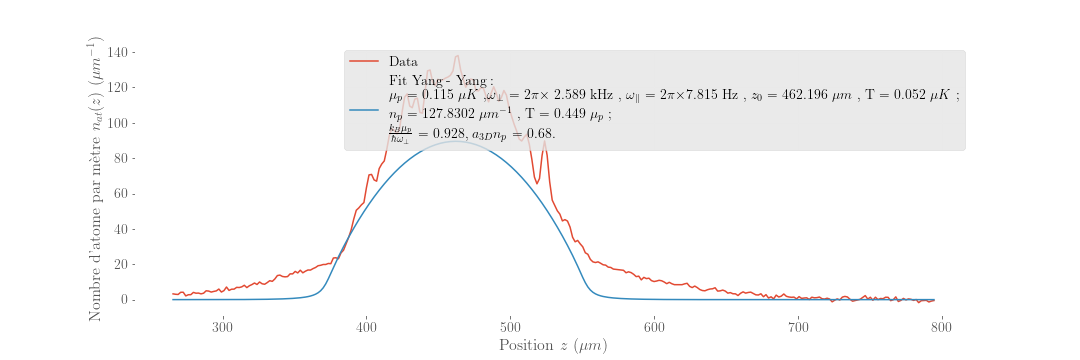
\includegraphics[width=0.99\textwidth]{n_at_2023-05-02-Scan-29_Y_Y_T}
		\end{column}


		
	\end{columns}
	}
	

	\only<3>{
	{~}\\
	{$\bullet$ Paramètres libres ${\color{red} \omega_\parallel} , {\color{red}T} $ }
	\begin{columns}
	
		\begin{column}{0.3\linewidth}
			$$ 
			{\tiny
			\begin{array}{rrl}
				\hline
				\hline
				\mu_p:  & 0.115 & \mu K\\
				\omega_\perp :  & 2 \pi  \times  2.589 & kHz	\\
				{\color{red} \omega_\parallel :}  & {\color{red} 2 \pi  \times 6.444}  & {\color{red} Hz	}\\
				z_0 :  & 462.19  & \mu m	\\
				{\color{red} T : } & {\color{red} 0.141  } & {\color{red} \mu K}\\			
				\hline
				\hline
				n_p :   &  127.83  & {\mu m}^{-1}\\	
				{\color{magenta} T : } & {\color{magenta} 1.22  } & {\color{magenta}\mu_p} \\				
				\hline
				\hline	
				\frac{ k_B \mu_p}{\hbar \omega_\perp } :  & 0.928  & 	\\
				n_p a_{3D} :  &  0.68  &  \\
				\hline
				\hline	
			\end{array}
			}
			$$


		\end{column}
		
		\begin{column}{0.7\linewidth}
			\centering
			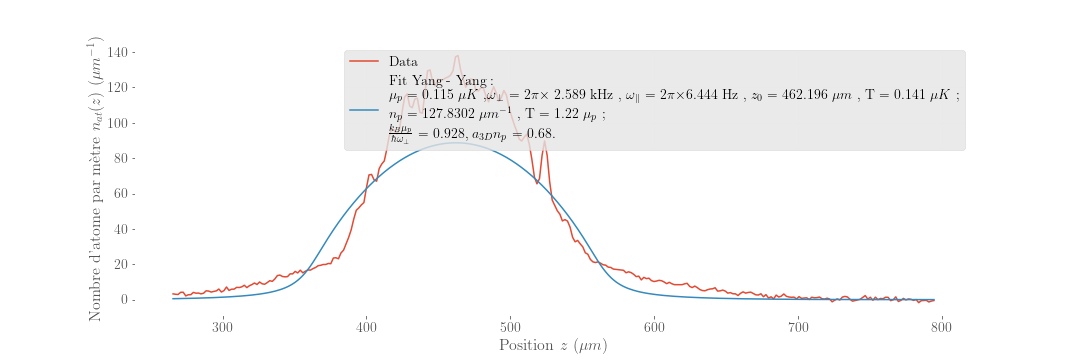
\includegraphics[width=0.99\textwidth]{n_at_2023-05-02-Scan-29_Y_Y_flong_T.png}	
		\end{column}


		
	\end{columns}
		
	{~}\\
	{~}\\
	{$\bullet$ Parametres libres ${\color{red} \omega_\parallel} , {\color{red} T}  , {\color{red} \mu_p} $ }

	\begin{columns}
	
		\begin{column}{0.3\linewidth}
			$$ 
			{\tiny
			\begin{array}{rrl}
				\hline
				\hline
				{\color{red} \mu_p :}   & {\color{red} 0.182 }  & {\color{red} \mu K}\\
				\omega_\perp :  & 2 \pi  \times  2.589  & kHz	\\
				{\color{red} \omega_\parallel :}  & {\color{red} 2 \pi  \times 10.131}  & {\color{red} Hz	}\\
				z_0 :  &  462.19  & \mu m	\\
				{\color{red} T : } & {\color{red} 0.824  } & {\color{red} \mu K}\\			
				\hline
				\hline
				{\color{magenta} n_p :  } & {\color{magenta} 239.12}  & {\color{magenta}{\mu m}^{-1}}\\	
				{\color{magenta} T : } & {\color{magenta} 4.522  } & {\color{magenta}\mu_p} \\				
				\hline
				\hline	
				{\color{magenta} \frac{ k_B \mu_p}{\hbar \omega_\perp } : } & {\color{magenta} 1.466}  & \\
				{\color{magenta} n_p a_{3D} : }  & {\color{magenta}  1.27}  &  \\
				\hline
				\hline	
			\end{array}
			}
			$$


		\end{column}
		
		\begin{column}{0.7\linewidth}
			\centering
			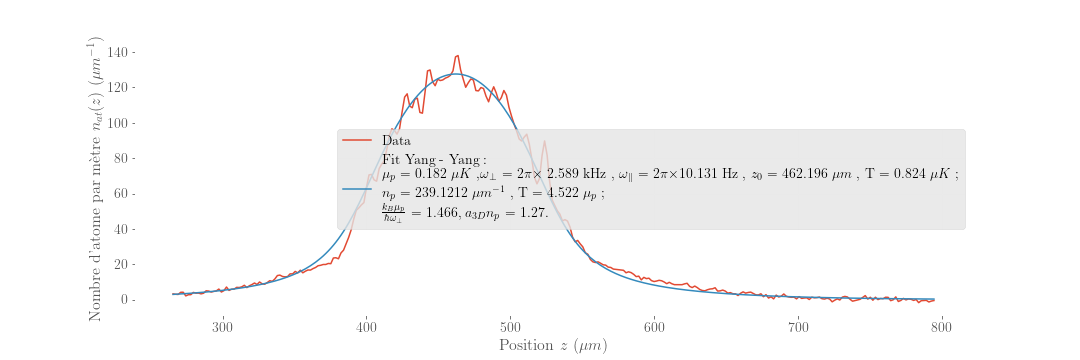
\includegraphics[width=0.99\textwidth]{n_at_2023-05-02-Scan-29_Y_Y_flong_T_mup.png}	
		\end{column}


		
	\end{columns}
	}
		
	\only<4>{
	{~}\\
	
	{$\bullet$ Paramètres libres $ {\color{red} \omega_\perp }, {\color{red} \omega_\parallel}  ,  {\color{red}T } , {\color{red}\mu_p }$}
	\begin{columns}
		
		\begin{column}{0.3\linewidth}
			$$ 
			{\tiny
			\begin{array}{rrl}
				\hline
				\hline
				{\color{red} \mu_p:}  & {\color{red} 0.116}  & {\color{red} \mu K}\\
				{\color{red} \omega_\perp : } & {\color{red} 2 \pi  \times 1.943}  & {\color{red} kHz} 	\\
				{\color{red} \omega_\parallel :}  & {\color{red} 2 \pi  \times 7.954}  & {\color{red} Hz	}\\
				z_0 :  & 462.19 &  \mu m	 \\
				{\color{red} T : } & {\color{red} 0.583   } & {\color{red} \mu K}\\			
				\hline
				\hline
				{\color{magenta} n_p :  } & {\color{magenta} 189.15}   & {\color{magenta} {\mu m}^{-1}}\\	
				{\color{magenta} T : } & {\color{magenta}  5.04 } & {\color{magenta}\mu_p} \\				
				\hline
				\hline	
				{\color{magenta} \frac{ k_B \mu_p}{\hbar \omega_\perp } : } & {\color{magenta} 1.24}  & 	\\
				{\color{magenta} n_p a_{3D} : }  & {\color{magenta} 1.0}  &  \\
				\hline
				\hline	
			\end{array}
			}
			$$


		\end{column}
		
		\begin{column}{0.7\linewidth}
			\centering
			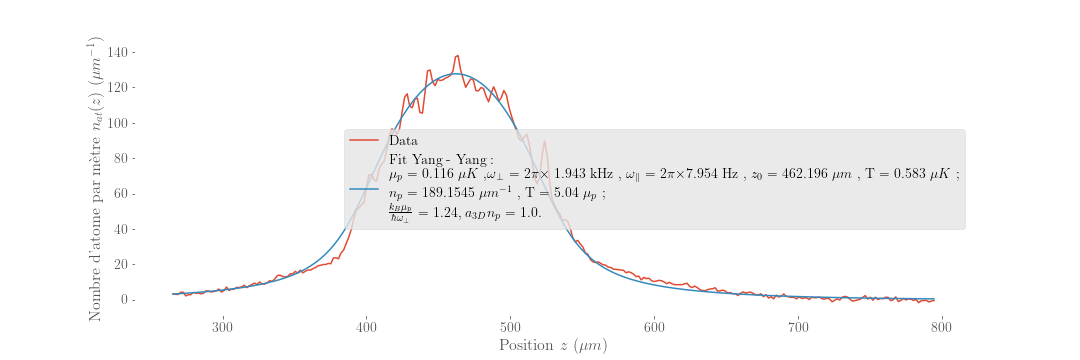
\includegraphics[width=0.99\textwidth]{n_at_2023-05-02-Scan-29_Y_Y_fperp_flong_T_mup}\\		
		\end{column}


		
	\end{columns}
		
	{~}\\
	{~}\\
	{$\bullet$ Paramètres libres ${\color{red} \omega_\perp}, {\color{red} \omega_\parallel} , {\color{red} z_0} ,  {\color{red}T}  , {\color{red}\mu_p }$ }

	\begin{columns}
	
		\begin{column}{0.3\linewidth}
			$$ 
			{\tiny
			\begin{array}{rrl}
				\hline
				\hline
				{\color{red} \mu_p:}  & {\color{red} 0.074}  & {\color{red} \mu K}\\
				{\color{red}\omega_\perp : } & {\color{red} 2 \pi  \times  1.671} & {\color{red}kHz	}\\
				{\color{red} \omega_\parallel :}  & {\color{red} 2 \pi  \times 6.164}  & {\color{red} Hz	}\\
				{\color{red} z_0 : } & {\color{red} 464.429 }& {\color{red} \mu m	} \\
				{\color{red} T : } & {\color{red} 0.391  } & {\color{red} \mu K}\\			
				\hline
				\hline
				{\color{magenta} n_p :   }& {\color{magenta} 127.65}  & {\color{magenta} {\mu m}^{-1}} \\	
				{\color{magenta} T : } & {\color{magenta} 5.268} & {\color{magenta}\mu_p} \\				
				\hline
				\hline	
				{\color{magenta} \frac{ k_B \mu_p}{\hbar \omega_\perp } : } & {\color{magenta} 0.927}  & 	\\
				{\color{magenta} n_p a_{3D} : }  & {\color{magenta} 0.68}  &  \\
				\hline
				\hline	
			\end{array}
			}
			$$


		\end{column}
		
		\begin{column}{0.7\linewidth}
			\centering
			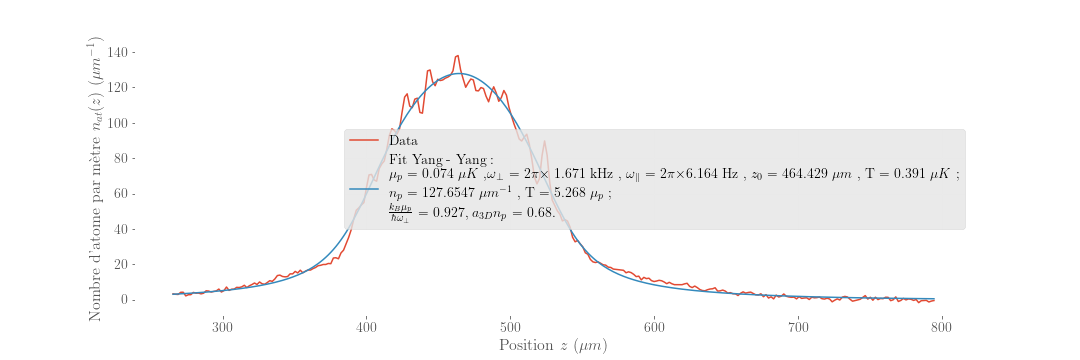
\includegraphics[width=0.9\textwidth]{n_at_2023-05-02-Scan-29_Y_Y_fperp_flong_x0_T_mup}		
		\end{column}

		
	\end{columns}
	}
	
	
	\only<5>{
	
	{~}\\
	{$\bullet$ Paramètres libres ${\color{red} \omega_\perp}, {\color{red} \omega_\parallel} , {\color{red} z_0} ,  {\color{red}T}  , {\color{red}\mu_p }$ }

	\begin{columns}
	
		\begin{column}{0.3\linewidth}
			$$ 
			{\tiny
			\begin{array}{rrl}
				\hline
				\hline
				{\color{red} \mu_p:}  & {\color{red} 0.115}  & {\color{red} \mu K}\\
				{\color{red}\omega_\perp : } & {\color{red} 2 \pi  \times  2.000} & {\color{red}kHz	}\\
				{\color{red} \omega_\parallel :}  & {\color{red} 2 \pi  \times 7.815}  & {\color{red} Hz	}\\
				{\color{red} z_0 : } & {\color{red} 464.43}& {\color{red} \mu m	} \\
				{\color{red} T : } & {\color{red} 0.405  } & {\color{red} \mu K}\\			
				\hline
				\hline
				{\color{magenta} n_p :   }& {\color{magenta} 180.90}  & {\color{magenta} {\mu m}^{-1}} \\	
				{\color{magenta} T : } & {\color{magenta} 3.519} & {\color{magenta}\mu_p} \\				
				\hline
				\hline	
				{\color{magenta} \frac{ k_B \mu_p}{\hbar \omega_\perp } : } & {\color{magenta} 1.2}  & 	\\
				{\color{magenta} n_p a_{3D} : }  & {\color{magenta} 0.96}  &  \\
				\hline
				\hline	
			\end{array}
			}
			$$


		\end{column}
		
		\begin{column}{0.7\linewidth}
			\centering
			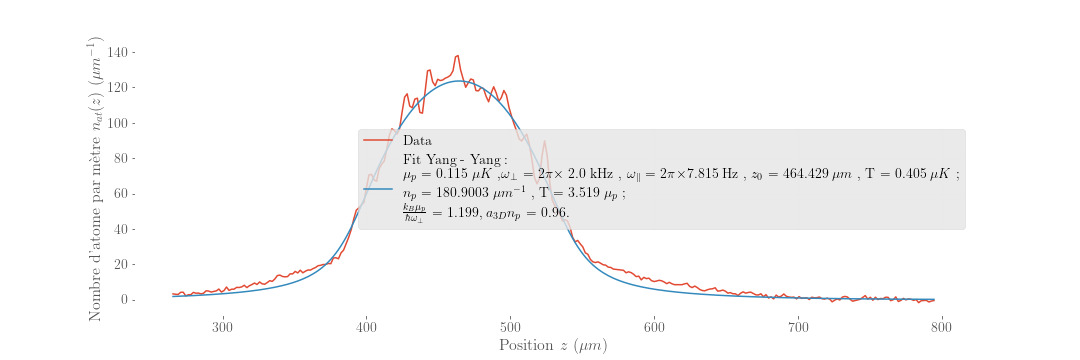
\includegraphics[width=0.9\textwidth]{n_at_2023-05-02-Scan-29_Y_Y_fperp_flong_x0_T_mup_2}		
		\end{column}

		
	\end{columns}
		
	}
	
\end{frame}

\begin{frame}[shrink=1]{Yang-Yang modifié}
	
	\only<1>{

	\begin{itemize}
		\item[Attente :]  Le paramètre $T$ sufisait pour fait un ajustement
		\item[ {\color{red} Pb \Frowny :}] 
			\begin{itemize}
				\item[$\bullet$] $T$ libre ne suffis pas
				\item[$\bullet$] L'ajustement se fait avec des valeurs different selon les paramètres libres
				\item[$\bullet$] les valeurs ajusté "Thomas-Fermi" et "Yang-Yang" sont différentes (même $n_p$ !!!) 
			\end{itemize}
		
		\item[ {\color{green} Idée \Smiley:} ]	Yang-Yang modifié [Bess]
			\begin{itemize}
				\item[$\rhd$] Prendre en compte que des atomes peuvent peupler des états transvers exités [Léa]
			\end{itemize}
			
		\item[ Action !!!]
			\begin{itemize}
			 	\item[$\rhd$] On constant durent les ajustement precedents que les paramètre sont très corrélés ;
			 		\begin{itemize}
			 			\item[$\bullet$] Avec Yang-Yang modifié  produire des profile longitudinal avec $T$ et $\mu_p$ différents ($\mu_p$ , $\omega_\perp$ et $\omega_\paralle$ fixes)
			 			\item[$\bullet$] Avec ajustement "Thomas-Fermi" mesurer $n_p$ et $\omega$
			 		\end{itemize} 
			 	\item[$\rhd$] Ajustement "Yang-Yang" modifié
			\end{itemize}
	\end{itemize} 	
	
	}
	
	\only<2>{
	\centering
	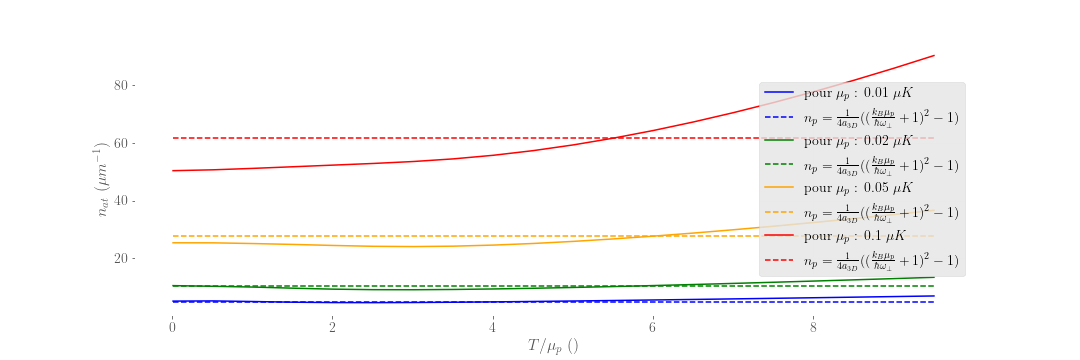
\includegraphics[width=0.9\textwidth]{n_p_2023-05-02-Scan-29_Y_Y_Modifed_T_mup}
	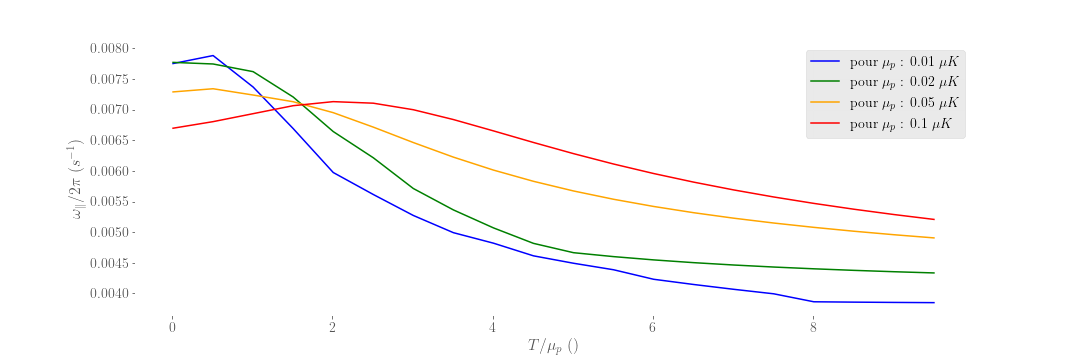
\includegraphics[width=0.9\textwidth]{omega_long_2023-05-02-Scan-29_Y_Y_Modifed_T_mup}
	}
		

\end{frame}


\begin{frame}[shrink=1]{Données du 2023-05-02-Scan-29 fit Yang-Yang modifié }
	
	\only<1>{
	{~}\\
	{~}\\
	{$\bullet$ Paramètre libre {\color{red}$ T $}}
	\begin{columns}
	
		\begin{column}{0.3\linewidth}
			$$ 
			{\tiny 
			\begin{array}{rrl}
				\hline
				\hline
				\mu_p:  &  0.141  & \mu K\\
				\omega_\perp :  & 2 \pi  \times  2.6  & kHz	\\
				\omega_\parallel :  & 2 \pi  \times  9.5 & Hz	\\
				z_0 :  &  462.19 & \mu m	\\
				{\color{red} T : } & {\color{red}   } & {\color{red} \mu K}\\			
				\hline
				\hline
				n_p :   &  166.87  & {\mu m}^{-1}\\	
				{\color{magenta} T : } & {\color{magenta}   } & {\color{magenta}\mu_p} \\				
				\hline
				\hline	
				\frac{ k_B \mu_p}{\hbar \omega_\perp } :  & 1.13  & 	\\
				n_p a_{3D} :  &  0.88  &  \\
				\hline
				\hline	
			\end{array}
			}
			$$


		\end{column}
		
		\begin{column}{0.7\linewidth}
			\centering
			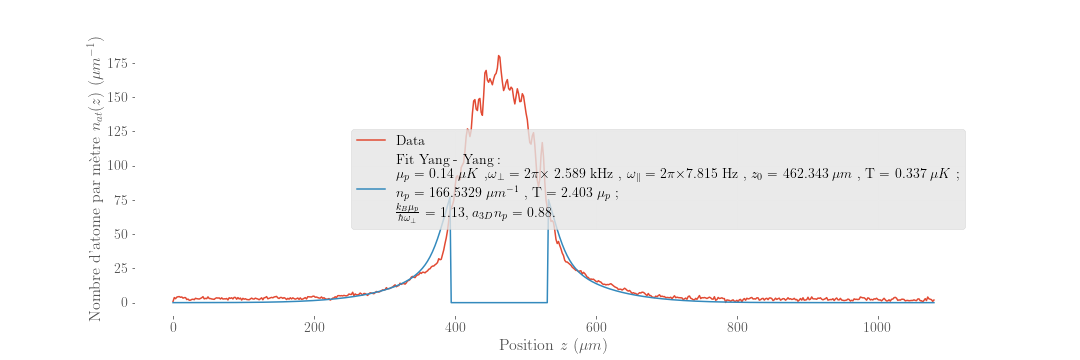
\includegraphics[width=0.99\textwidth]{n_at_2023-05-02-Scan-29_Y_Y_Modifed_T}
		\end{column}


		
	\end{columns}
	
	

	{~}\\
	{$\bullet$ Paramètres libres $ {\color{red}T} , {\color{red} \mu_p}  $ }
	\begin{columns}
	
		\begin{column}{0.3\linewidth}
			$$ 
			{\tiny
			\begin{array}{rrl}
				\hline
				\hline
				{\color{red} \mu_p : }  & {\color{red}  } & {\color{red} \mu K }\\
				\omega_\perp :  & 2 \pi  \times  2.6 & kHz	\\
				 \omega_\parallel : & 2 \pi \times 9.5  &  Hz	\\
				z_0 :  & 462.19  & \mu m	\\
				{\color{red} T : } & {\color{red} 0.5414 } & {\color{red} \mu K}\\			
				\hline
				\hline
				{\color{magenta} n_p : }  &  {\color{magenta} 166.87 } & {\color{magenta} {\mu m}^{-1}}\\	
				{\color{magenta} T : } & {\color{magenta} 3.855  } & {\color{magenta}\mu_p} \\				
				\hline
				\hline	
				{\color{magenta} \frac{ k_B \mu_p}{\hbar \omega_\perp } : } & {\color{magenta} 1.13 } & 	\\
				{\color{magenta} n_p a_{3D} :}  &  {\color{magenta} 0.88}  &  \\
				\hline
				\hline	
			\end{array}
			}
			$$


		\end{column}
		
		\begin{column}{0.7\linewidth}
			\centering
			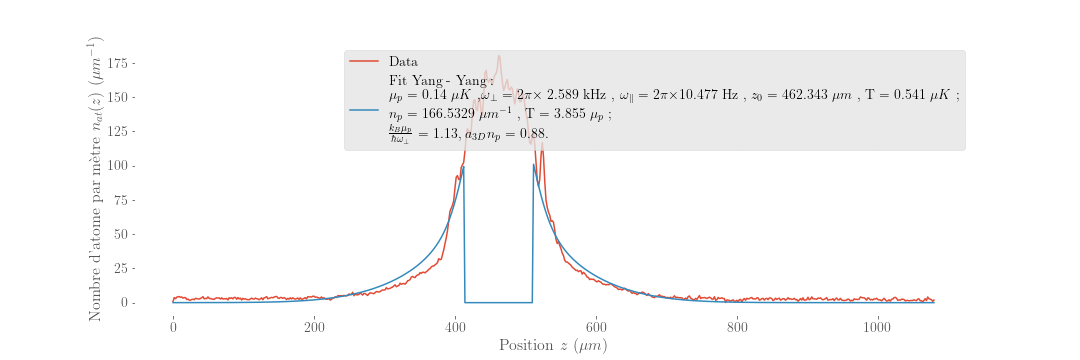
\includegraphics[width=0.99\textwidth]{n_at_2023-05-02-Scan-29_Y_Y_Modifed_flong_T.png}	
		\end{column}


		
	\end{columns}
		
	}
		

	
\end{frame}



